\documentclass[11pt,a4paper]{article}

\usepackage[top=2cm, bottom=2cm, left=2cm, right=2cm]{geometry}

\usepackage{amsmath,amssymb}
\usepackage{graphicx}
\usepackage{float}
\usepackage{algorithm}
\usepackage{algpseudocode}
\usepackage{booktabs}
\usepackage{hyperref}
\usepackage{times}
\usepackage{tikz}
\usetikzlibrary{arrows.meta,positioning}

\title{\vspace{-1cm}\textbf{Multi-Restart Simulated Annealing for Neural Network Policy Optimisation in Inventory Management}\vspace{-0.25cm}}
\author{Hammerschmidt, Jakob Elias \and Al Hachem, Marc \and Elmehelmy, Seif Ahmed Moheb}
\date{}

\begin{document}
\maketitle

\section{Big Picture and Intuition}

Inventory management in multi-echelon supply chains is a difficult problem due to stochastic demand, delayed order arrivals, and competing cost objectives. The goal is to learn an ordering policy that maximises cumulative profit by balancing holding costs, ordering costs, and lost sales penalties.

We formulate this as a policy optimisation problem where a neural network maps inventory states to ordering decisions. The main difficulty is that the reward landscape is noisy (due to stochastic demand) and multimodal (multiple local optima exist for different ordering strategies).

\textbf{Why Simulated Annealing over Policy Gradients.}
Traditional reinforcement learning methods like REINFORCE compute gradient estimates from sampled trajectories. In our experiments, these gradient signals proved unreliable: the high variance from stochastic demand caused unstable learning, converging to suboptimal policies around reward $\approx 7800$. Simulated Annealing (SA), being derivative-free, avoids this by treating the neural network weights as a black-box optimisation problem.

\textbf{The Multi-Restart Strategy.}
Single SA runs frequently converged to local optima around reward $\approx 7000$. The solution landscape contains multiple basins of attraction, and escaping them requires more than temperature-based exploration. We therefore use multiple independent SA restarts with a dynamic exploration--exploitation schedule: early restarts explore the parameter space with random initialisation, while later restarts exploit by refining the best solution found so far. This achieves rewards $>10{,}000$.

\section{Methodology}
\subsection{Problem Formulation}

We model the decision-making policy as a neural network $\pi_\theta$ with approximately 500 parameters. The policy maps the environment state (inventory levels and day of week) to order quantities. Since the environment requires integer actions, the continuous outputs are floored.

The objective is to maximise total profit over an episode of length $T = 28$ days:
\begin{equation}
\theta^* = \arg\max_{\theta} \; \mathbb{E}\left[\sum_{t=1}^{T} r_t \right],
\end{equation}
where $r_t$ is the profit at time step $t$.

\subsection{Simulated Annealing with Gaussian Perturbations}

We optimise $\theta$ using Simulated Annealing (SA). At each iteration, a candidate solution is generated by adding Gaussian noise:
\begin{equation}
\theta' = \theta + \epsilon, \quad \epsilon \sim \mathcal{N}(0, \sigma^2 I).
\end{equation}
The perturbation scale $\sigma$ decreases linearly from 0.4 to 0.2 within each restart, so we explore broadly first, then refine.

Candidates are accepted using the Metropolis criterion:
\begin{equation}
P(\text{accept}) =
\begin{cases}
1, & \text{if } \Delta > 0, \\
\exp(\Delta / T_k), & \text{otherwise},
\end{cases}
\end{equation}
where $\Delta = J(\theta') - J(\theta)$ and $T_k = T_0/(1 + 0.5k)$ with $T_0 = 5 \times 10^5$.

\subsection{Multi-Restart Strategy}

To avoid poor local optima, we use $N = 10$ restarts, each allocated an equal share of the episode budget. The probability of exploration decreases over restarts:
\begin{equation}
P(\text{explore})_i = 0.8 - 0.6 \cdot \frac{i}{N}.
\end{equation}
The first restart uses the initial policy, while subsequent exploration restarts use Xavier initialisation. Later restarts exploit the best policy found so far using small perturbations ($\sigma = 0.05$).

\subsection{Variance Reduction}

Single-episode evaluations are noisy due to stochastic demand. We evaluate each policy using the mean return over $n = 5$ episodes, which reduces variance and gives more reliable acceptance decisions.

\section{Pseudocode}

\begin{algorithm}[H]
\caption{Multi-Restart Simulated Annealing for Policy Optimisation}
\begin{algorithmic}[1]
\Require Environment $\mathcal{E}$, policy network $\pi_\theta$, budget $B$, restarts $N$
\Ensure Optimised parameters $\theta^*$
\State $\theta^* \gets \text{None}$, $J^* \gets -\infty$
\For{$i = 1$ to $N$}
    \State $p_{\text{explore}} \gets 0.8 - 0.6 \cdot i/N$
    \If{$i = 1$ \textbf{or} $\text{rand}() < p_{\text{explore}}$}
        \State $\theta \gets \text{XavierInit}()$ \Comment{Exploration: random start}
    \Else
        \State $\theta \gets \theta^* + \mathcal{N}(0, 0.05^2 I)$ \Comment{Exploitation: refine best}
    \EndIf
    \State $\theta_{\text{best}} \gets \theta$, $J_{\text{best}} \gets \text{Evaluate}(\theta, \mathcal{E}, n=5)$
    \State $J \gets J_{\text{best}}$ \Comment{Current reward for Metropolis}
    \For{$k = 1$ to $K$} \Comment{SA iterations within restart}
        \State $\sigma \gets 0.4 \cdot (1 - 0.5 \cdot k/K)$ \Comment{Adaptive step size}
        \State $\theta' \gets \theta + \mathcal{N}(0, \sigma^2 I)$
        \State $J' \gets \text{Evaluate}(\theta', \mathcal{E}, n=5)$
        \If{$J' > J_{\text{best}}$}
            \State $\theta_{\text{best}} \gets \theta'$, $J_{\text{best}} \gets J'$
        \EndIf
        \State $\Delta \gets J' - J$, $T \gets T_0 / (1 + 0.5k)$
        \If{$\Delta > 0$ \textbf{or} $\text{rand}() < \exp(\Delta / T)$}
            \State $\theta \gets \theta'$, $J \gets J'$ \Comment{Metropolis acceptance}
        \EndIf
    \EndFor
    \If{$J_{\text{best}} > J^*$}
        \State $\theta^* \gets \theta_{\text{best}}$, $J^* \gets J_{\text{best}}$
    \EndIf
\EndFor
\State \Return $\theta^*$
\end{algorithmic}
\end{algorithm}

\begin{figure}[h]
    \centering
    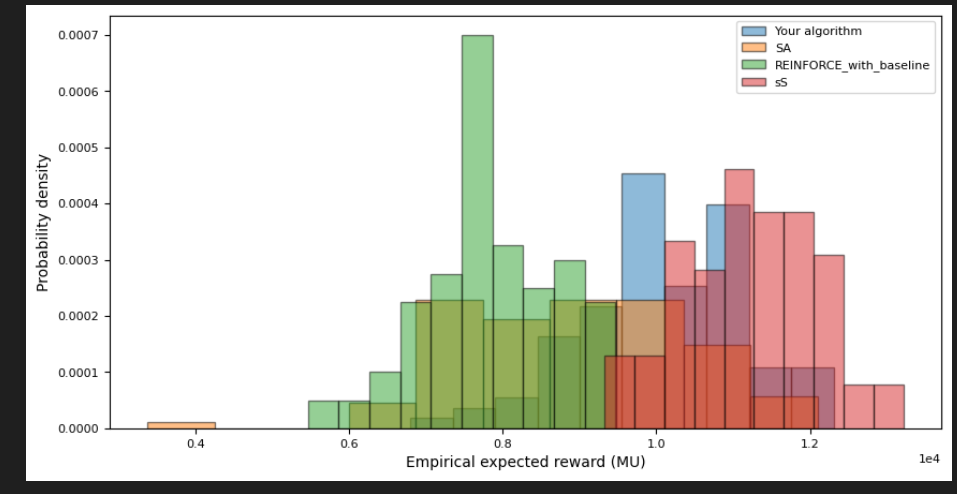
\includegraphics[width=0.85\textwidth]{figures/performance_comparison.png}
    \caption{Distribution of episodic rewards across 100 test scenarios. Our Multi-Restart SA (blue) achieves mean reward $\approx 10{,}100$, outperforming vanilla SA ($\approx 8{,}900$) and REINFORCE with baseline ($\approx 7{,}800$). The (s,S) heuristic (red) provides an upper bound at $\approx 11{,}200$ but requires domain-specific policy structure.}
    \label{fig:comparison}
\end{figure}

\begin{figure}[h]
    \centering
    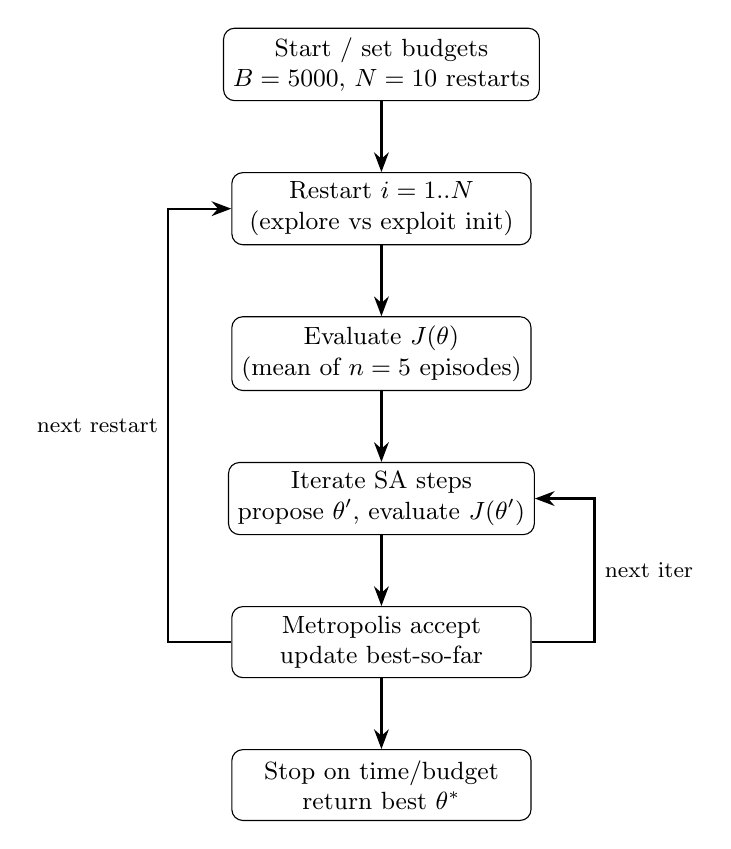
\begin{tikzpicture}[
        node distance=0.9cm,
        box/.style={rectangle, rounded corners, draw, minimum width=3.8cm, minimum height=0.9cm, align=center, font=\small},
        arrow/.style={-{Stealth[length=2.5mm]}, thick}
    ]
        \node[box] (start) {Start / set budgets\\$B=5000$, $N=10$ restarts};
        \node[box, below=of start] (restart) {Restart $i = 1..N$\\(explore vs exploit init)};
        \node[box, below=of restart] (eval) {Evaluate $J(\theta)$\\(mean of $n=5$ episodes)};
        \node[box, below=of eval] (sa) {Iterate SA steps\\propose $\theta'$, evaluate $J(\theta')$};
        \node[box, below=of sa] (metro) {Metropolis accept\\update best-so-far};
        \node[box, below=of metro] (stop) {Stop on time/budget\\return best $\theta^*$};

        \draw[arrow] (start) -- (restart);
        \draw[arrow] (restart) -- (eval);
        \draw[arrow] (eval) -- (sa);
        \draw[arrow] (sa) -- (metro);
        \draw[arrow] (metro) -- (stop);

        \draw[arrow] (metro.east) -- ++(0.8,0) |- node[right, pos=0.25, font=\footnotesize] {next iter} (sa.east);
        \draw[arrow] (metro.west) -- ++(-0.8,0) |- node[left, pos=0.25, font=\footnotesize] {next restart} (restart.west);
    \end{tikzpicture}
    \caption{High-level flow of the multi-restart simulated annealing policy search.}
    \label{fig:blockdiagram}
\end{figure}
\newpage

\begin{thebibliography}{9}
\bibitem{kirkpatrick1983}
Kirkpatrick, S., Gelatt, C. D., \& Vecchi, M. P. (1983). Optimization by simulated annealing. \textit{Science}, 220(4598), 671--680.

\bibitem{williams1992}
Williams, R. J. (1992). Simple statistical gradient-following algorithms for connectionist reinforcement learning. \textit{Machine Learning}, 8(3), 229--256.

\bibitem{salimans2017}
Salimans, T., Ho, J., Chen, X., Sidor, S., \& Sutskever, I. (2017). Evolution strategies as a scalable alternative to reinforcement learning. \textit{arXiv:1703.03864}.

\bibitem{Glorot2010}
Glorot, X., \& Bengio, Y. (2010). Understanding the difficulty of training deep feedforward neural networks. \textit{AISTATS}.

\bibitem{PseudocodeConvention}
University of Waterloo. CS 231 Pseudocode Convention. \\
\url{https://student.cs.uwaterloo.ca/~cs231/resources/pseudocode.pdf}
\end{thebibliography}

\end{document}
